
\documentclass{article}[14pt]
\usepackage{multicol, enumerate, enumitem, hyperref, color, soul, setspace, parskip, fancyhdr, amssymb, amsthm, amsmath, bbm, latexsym, units, mathtools}
\everymath{\displaystyle}
\usepackage[headsep=0.5cm,headheight=0cm, left=1 in,right= 1 in,top= 1 in,bottom= 1 in]{geometry}
\pagestyle{fancy}
\lhead{}
\chead{Answer Key for Module\,6\,-\,Polynomial\,Functions Version B}
\rhead{}
\lfoot{Summer\,C\,2020}
\cfoot{}
\rfoot{}
\begin{document}
\textbf{This key should allow you to understand why you choose the option you did (beyond just getting a question right or wrong). \href{https://xronos.clas.ufl.edu/mac1105spring2020/courseDescriptionAndMisc/Exams/LearningFromResults}{More instructions on how to use this key can be found here}.}

\textbf{If you have a suggestion to make the keys better, \href{https://forms.gle/CZkbZmPbC9XALEE88}{please fill out the short survey here}.}

\textit{Note: This key is auto-generated and may contain issues and/or errors. The keys are reviewed after each exam to ensure grading is done accurately. If there are issues (like duplicate options), they are noted in the offline gradebook. The keys are a work-in-progress to give students as many resources to improve as possible.}

\rule{\textwidth}{0.4pt}

26. Construct the lowest-degree polynomial given the zeros below. Then, choose the intervals that contain the coefficients of the polynomial in the form $x^3+bx^2+cx+d$.
$$ -5 + 2i \text{ and } -3 $$ 
The solution is $ x^{3} +13 x^{2} +59 x + 87 $ 

\begin{enumerate}[label=\Alph*.] 
\item $ b \in [-2, 2], c \in [-2, 3], \text{ and } d \in [-7, -5] $ 

 $x^{3} + x^{2} +x -6$, which corresponds to multiplying out $(x -2)(x + 3)$. 
\item $ b \in [10, 18], c \in [52, 65], \text{ and } d \in [82, 88] $ 

 * $x^{3} +13 x^{2} +59 x + 87$, which is the correct option. 
\item $ b \in [-18, -10], c \in [52, 65], \text{ and } d \in [-91, -86] $ 

 $x^{3} -13 x^{2} +59 x -87$, which corresponds to multiplying out $(x-(-5 + 2i))(x-(-5 - 2i))(x -3)$. 
\item $ b \in [-2, 2], c \in [3, 10], \text{ and } d \in [7, 18] $ 

 $x^{3} + x^{2} +8 x + 15$, which corresponds to multiplying out $(x + 5)(x + 3)$. 
\item $ \text{None of the above.} $ 

 This corresponds to making an unanticipated error or not understanding how to use nonreal complex numbers to create the lowest-degree polynomial. If you chose this and are not sure what you did wrong, please contact the coordinator for help. 
\end{enumerate} 
 
General Comments: Remember that the conjugate of $a+bi$ is $a-bi$. Since these zeros always come in pairs, we need to multiply out $(x-(-5 + 2i))(x-(-5 - 2i))(x-(-3))$.

-----------------------------------------------

27. Describe the end behavior of the polynomial below.
$$ f(x) = 4(x - 6)^{3}(x + 6)^{4}(x - 8)^{3}(x + 8)^{4} $$ 

 
 The solution is  
 \begin{center} 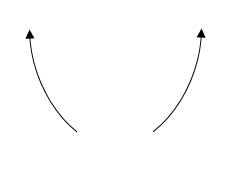
\includegraphics[width=0.3\textwidth]{../Figures/endBehaviorPositiveEvenB.png} \end{center}\begin{tabular}{|c|c|} 
\hline 
 & \tabularnewline 
 \textbf{A.} 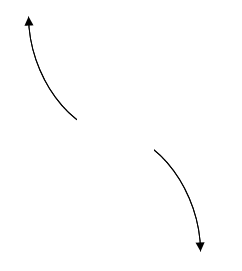
\includegraphics[width=0.3\textwidth]{../Figures/endBehaviorNegativeOddB.png} & \textbf{B.} 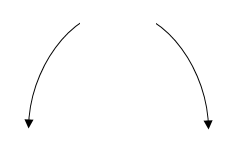
\includegraphics[width=0.3\textwidth]{../Figures/endBehaviorNegativeEvenB.png} \tabularnewline 
\hline 
 & \tabularnewline 
 \textbf{C.} 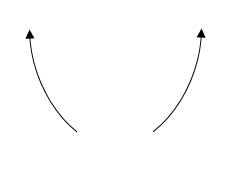
\includegraphics[width=0.3\textwidth]{../Figures/endBehaviorPositiveEvenB.png} & \textbf{D.} 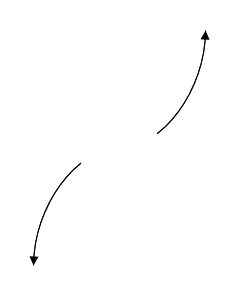
\includegraphics[width=0.3\textwidth]{../Figures/endBehaviorPositiveOddB.png} \tabularnewline 
\hline 
 E. None of the figures above. & \tabularnewline 
\hline 
 \end{tabular} 
 
\textbf{General Comments:} Remember that end behavior is determined by the leading coefficient AND whether the \textbf{sum} of the multiplicities is positive or negative.

-----------------------------------------------

28. Describe the zero behavior of the zero $x = -5$ of the polynomial below.
$$ f(x) = -4(x - 8)^{10}(x + 8)^{7}(x - 5)^{12}(x + 5)^{9} $$ 

 
 The solution is  
 \begin{center} 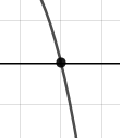
\includegraphics[width=0.3\textwidth]{../Figures/zeroBehaviorNegativeOddB.png} \end{center}\begin{tabular}{|c|c|} 
\hline 
 & \tabularnewline 
 \textbf{A.} 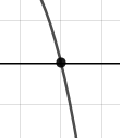
\includegraphics[width=0.3\textwidth]{../Figures/zeroBehaviorNegativeOddB.png} & \textbf{B.} 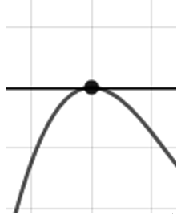
\includegraphics[width=0.3\textwidth]{../Figures/zeroBehaviorNegativeEvenB.png} \tabularnewline 
\hline 
 & \tabularnewline 
 \textbf{C.} 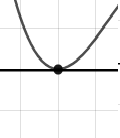
\includegraphics[width=0.3\textwidth]{../Figures/zeroBehaviorPositiveEvenB.png} & \textbf{D.} 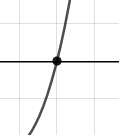
\includegraphics[width=0.3\textwidth]{../Figures/zeroBehaviorPositiveOddB.png} \tabularnewline 
\hline 
 E. None of the figures above. & \tabularnewline 
\hline 
 \end{tabular} 
 
\textbf{General Comments:} You will need to sketch the entire graph, then zoom in on the zero the question asks about.

-----------------------------------------------

29. Which of the following equations \textit{could} be of the graph presented below?
\begin{center} 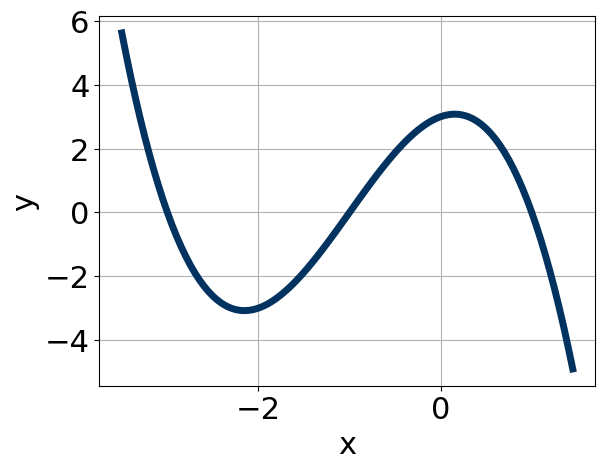
\includegraphics[width=0.3\textwidth]{../Figures/polyGraphToFunctionB.png} \end{center} 

The solution is $ 2(x - 1)^{7} (x + 1)^{9} (x + 3)^{11} $ 

\begin{enumerate}[label=\Alph*.] 
\item $ 2(x - 1)^{7} (x + 1)^{9} (x + 3)^{11} $ 

 * This is the correct option. 
\item $ 4(x - 1)^{4} (x + 1)^{10} (x + 3)^{7} $ 

 The factors $1$ and $-1$ have have been odd power. 
\item $ -17(x - 1)^{7} (x + 1)^{9} (x + 3)^{9} $ 

 This corresponds to the leading coefficient being the opposite value than it should be. 
\item $ 10(x - 1)^{4} (x + 1)^{11} (x + 3)^{5} $ 

 The factor $1$ should have been an odd power. 
\item $ -7(x - 1)^{6} (x + 1)^{7} (x + 3)^{11} $ 

 The factor $(x - 1)$ should have an odd power and the leading coefficient should be the opposite sign. 
\end{enumerate} 
 
General Comments: Draw the x-axis to determine which zeros are touching (and so have even multiplicity) or cross (and have odd multiplicity).

-----------------------------------------------

30. Construct the lowest-degree polynomial given the zeros below. Then, choose the intervals that contain the coefficients of the polynomial in the form $ax^3+bx^2+cx+d$.
$$ \frac{4}{5}, -7, \text{ and } -6 $$ 
The solution is $ 5x^{3} +61 x^{2} +158 x -168 $ 

\begin{enumerate}[label=\Alph*.] 
\item $ a \in [-6, 10], b \in [-4, 2], c \in [-216, -208], \text{ and } d \in [-178, -159] $ 

 $5x^{3} -1 x^{2} -214 x -168$, which corresponds to multiplying out $(5x + 5)(x + 1)(x -1)$. 
\item $ a \in [-6, 10], b \in [66, 79], c \in [260, 268], \text{ and } d \in [167, 174] $ 

 $5x^{3} +69 x^{2} +262 x + 168$, which corresponds to multiplying out $(5x + 5)(x -1)(x -1)$. 
\item $ a \in [-6, 10], b \in [57, 66], c \in [147, 159], \text{ and } d \in [167, 174] $ 

 $5x^{3} +61 x^{2} +158 x + 168$, which corresponds to multiplying everything correctly except the constant term. 
\item $ a \in [-6, 10], b \in [-64, -59], c \in [147, 159], \text{ and } d \in [167, 174] $ 

 $5x^{3} -61 x^{2} +158 x + 168$, which corresponds to multiplying out $(5x + 4)(x -7)(x -6)$. 
\item $ a \in [-6, 10], b \in [57, 66], c \in [147, 159], \text{ and } d \in [-178, -159] $ 

 * $5x^{3} +61 x^{2} +158 x -168$, which is the correct option. 
\end{enumerate} 
 
General Comments: To construct the lowest-degree polynomial, you want to multiply out $(5x -4)(x + 7)(x + 6)$

-----------------------------------------------


\end{document}

